
\ECchapter{01}{Renewable Energy}{Can solar power meet tomorrow's energy needs?}{ECOrange}

\ECObjectives{
\begin{itemize}[leftmargin=*,itemsep=1pt,topsep=1pt]
\item Explain how a photovoltaic cell and a grid-connected PV system operate.
\item Interpret capacity data and calculate annual additions.
\item Discuss intermittency, storage, grid integration and recycling.
\end{itemize}
}

\begin{multicols}{2}

\begin{engineeringnews}
Global renewable capacity grew by a record 692 GW in 2025. Solar power alone
accounted for about 510 GW of additions, nearly three-quarters of the renewable
total. The engineering challenge is now not only to manufacture more panels, but
also to connect variable generation to stronger and more flexible grids.
\end{engineeringnews}

\begin{ecarticle}
A photovoltaic (PV) cell converts light directly into electricity. Most commercial
cells are manufactured from silicon, a semiconductor. When photons provide enough
energy, electrons can move through the material. The internal electric field of the
p--n junction separates the electrical charges and creates a direct current.

A PV module connects many cells together. Modules are combined into strings and
arrays to reach the required voltage and power. However, a module rarely operates at
a fixed point. Its voltage-current characteristic changes with solar irradiance and
temperature. A maximum power point tracker continuously adjusts the operating point
so that the array delivers as much power as possible.

The generated electricity is direct current, whereas buildings and public grids use
alternating current. An inverter therefore converts DC into AC, synchronises the
voltage and frequency with the grid, and provides protection and monitoring
functions. A battery may store surplus electricity, but it increases cost, material
use and conversion losses.

Solar power is variable: output changes with clouds, season and time of day. Engineers
integrate large amounts of PV using forecasting, flexible demand, interconnections,
storage and controllable generation. The objective is not to make every installation
independent, but to balance the complete electricity system.

The environmental impact of a PV system must be assessed over its entire life cycle.
Manufacturing requires energy and materials, while end-of-life modules contain glass,
aluminium, copper, polymers and semiconductor materials. Designing modules that are
efficient, durable, repairable and recyclable is therefore a major engineering goal.
\end{ecarticle}

\begin{figure}[H]
\centering
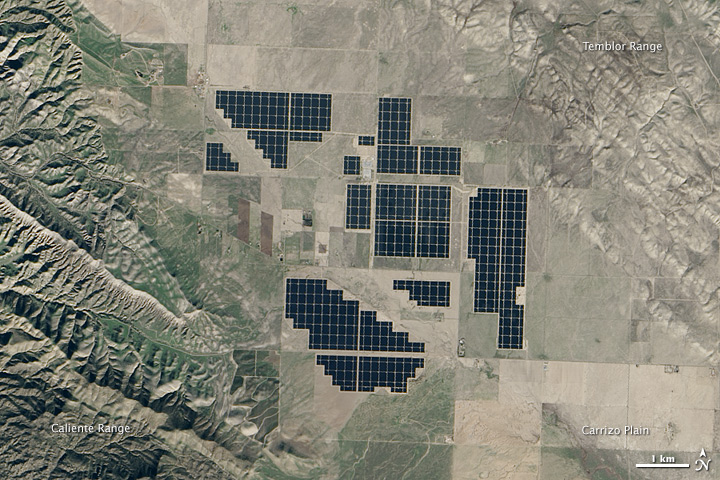
\includegraphics[width=\linewidth]{images/EC01/topaz_solar_farm.jpg}
\caption*{\footnotesize Topaz Solar Farm, California. NASA image, public domain.}
\end{figure}

\columnbreak

\begin{engineeringfocus}
\textbf{Designing a photovoltaic installation}

Engineers must optimise several parameters simultaneously:
\begin{itemize}[leftmargin=*,itemsep=1pt]
\item panel orientation and tilt;
\item inverter sizing and MPPT architecture;
\item cable cross-sections and electrical losses;
\item thermal behaviour and ventilation;
\item protection and isolation devices;
\item monitoring and maintenance strategy;
\item expected lifetime and recyclability.
\end{itemize}

A good design minimises the levelised cost of electricity while ensuring safety,
reliability and high annual energy yield.
\end{engineeringfocus}

\begin{figure}[H]
\centering
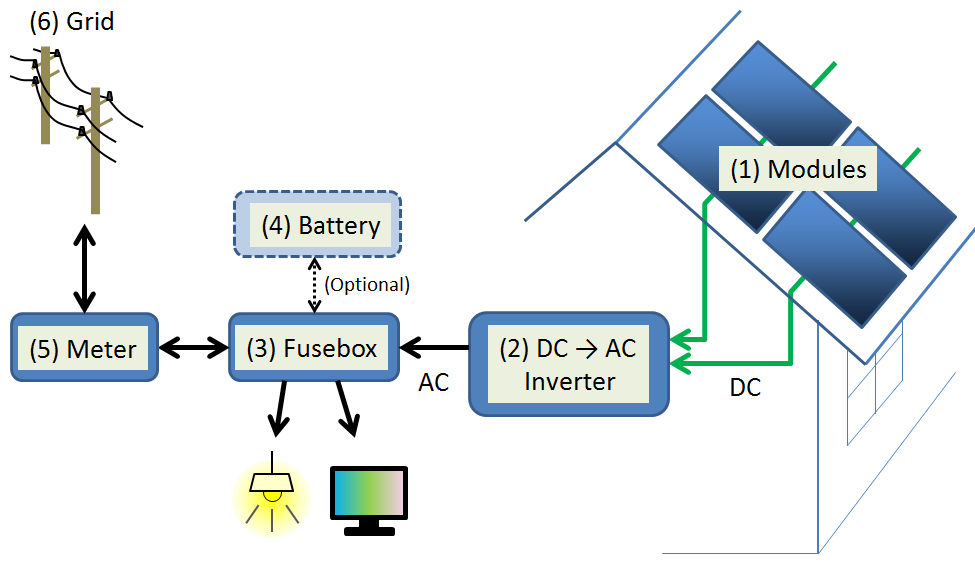
\includegraphics[width=\linewidth]{images/EC01/pv_system.png}
\caption*{\footnotesize Simplified residential PV system. S-kei, CC0.}
\end{figure}

\begin{tcolorbox}[colback=white,colframe=ECBlue,
title=\sffamily\bfseries Global solar PV capacity]
\centering
\begin{tikzpicture}
\begin{axis}[
width=\linewidth,height=47mm,
xlabel={Year},ylabel={Installed capacity (GW)},
xmin=2016,xmax=2025,ymin=0,ymax=2500,
xtick={2016,2018,2020,2022,2024},
grid=major,
tick label style={font=\scriptsize},
label style={font=\scriptsize},
]
\addplot+[mark=*,thick] table[x=year,y=capacity_gw,col sep=comma]
{data/EC01/global_solar_pv_capacity.csv};
\end{axis}
\end{tikzpicture}

{\scriptsize Source: IRENA, Renewable Capacity Statistics 2026.}
\end{tcolorbox}

\begin{tcolorbox}[colback=yellow!10,colframe=ECOrange,
title=\sffamily\bfseries Did You Know?]
The solar energy reaching the Earth in roughly one hour is comparable to humanity's
annual energy use. The main engineering challenge is therefore to capture, convert,
store and distribute only a small fraction of this resource efficiently.
\end{tcolorbox}

\begin{tcolorbox}[colback=ECLightBlue,colframe=ECBlue,
title=\sffamily\bfseries Key Figures]
\begin{tabularx}{\linewidth}{@{}Xr@{}}
Commercial module efficiency & 20--24\%\\
Typical module lifetime & 25--30 years\\
Typical inverter efficiency & 97--99\%\\
Annual module degradation & 0.3--0.5\%/year\\
Global PV capacity in 2025 & $\approx 2.4$ TW
\end{tabularx}
\end{tcolorbox}

\begin{vocabulary}
\begin{tabularx}{\linewidth}{@{}lX@{}}
solar cell & cellule photovoltaïque\\
irradiance & irradiance\\
inverter & onduleur\\
grid & réseau électrique\\
storage & stockage\\
yield & production énergétique\\
lifetime & durée de vie\\
recycling & recyclage
\end{tabularx}
\end{vocabulary}

\begin{questions}
\item Explain the role of the p--n junction.
\item Why does a PV installation need an inverter?
\item What is the purpose of MPPT control?
\item Use the graph to estimate the increase between 2020 and 2025.
\item Give three technical solutions for integrating variable solar power.
\item Why must environmental assessment include manufacturing and end-of-life?
\end{questions}

\begin{challenge}
Your school consumes 410 MWh of electricity each year and has 850 m$^2$ of usable
roof area. Prepare a preliminary PV study:
\begin{enumerate}[leftmargin=*,itemsep=1pt]
\item estimate the peak power that could be installed;
\item estimate annual energy production;
\item discuss the likely self-consumption ratio;
\item decide whether battery storage is justified;
\item propose useful monitoring indicators.
\end{enumerate}
Present your conclusions as a short engineering report.
\end{challenge}

\begin{applicationexercise}
A 420~W PV module receives an average irradiance of 850~W/m$^2$ over an active area of
2.0~m$^2$. Calculate its instantaneous efficiency. Then estimate the electrical energy
produced by 120 identical modules during 4.5 equivalent full-sun hours. State two reasons
why the real daily yield may be lower.
\end{applicationexercise}

\begin{speaking}
Working in pairs, prepare a five-minute presentation answering the question:
``Can Europe rely mainly on solar electricity by 2050?'' Support your arguments with
technical evidence, environmental impacts, economic considerations and examples from
different European countries.
\end{speaking}

\end{multicols}

